\section{Results}
\label{sec:results}

We report the one-versus-one adaptation ladder: static versus static,
static versus adaptive, adaptive versus static, adaptive versus
adaptive, and persistent versus persistent. All five cells share the
same seed, horizon and environment, so differences are attributable to
adaptation level. Language-model policies are not used in this section;
heuristic policies with a stealth (attacker) or vigilance (defender)
parameter occupy B1/B2, which is the correct first test of whether the
\emph{phenomenon} exists~\cite{rosin1997new}.

\subsection{Adaptation Changes Effectiveness (RQ1, H1)}
Table~\ref{tab:ladder} and Fig.~\ref{fig:ladder} summarise the ladder.

\begin{table}[!t]
\caption{One-versus-one adaptation ladder (40 episodes, seed 100).}
\label{tab:ladder}
\centering
\begin{tabular}{@{}lcccc@{}}
\toprule
\textbf{Matchup} & \textbf{ASR} & \textbf{DR} & \textbf{CEP} & \textbf{AG} \\
\midrule
Static / static         & $0.050$ & $0.975$ & $0.36$ & $0.000$ \\
Static / adaptive       & $0.050$ & $0.975$ & $0.42$ & $0.000$ \\
Adaptive / static       & $0.075$ & $0.550$ & $0.41$ & $0.025$ \\
Adaptive / adaptive     & $0.100$ & $0.550$ & $0.50$ & $0.050$ \\
Persistent / persistent & $0.075$ & $0.575$ & $0.47$ & $0.025$ \\
\bottomrule
\end{tabular}
\end{table}

A static attacker is almost always detected ($\mathrm{DR}=0.975$) and
rarely exfiltrates ($\mathrm{ASR}=0.05$), whether the defender adapts or
not. Giving the attacker episodic adaptation more than halves detection
($\mathrm{DR}=0.55$) and raises success. The mechanism is stealth
pacing: after a noisy exploit the attacker inserts waits so that
suspicion decays, a behaviour that the static policy never selects
because its stealth parameter never moves. H1 is supported for
detection and, more weakly, for success. An adaptive defender facing a
static attacker does not further reduce ASR: the static attacker is
already loud enough that the baseline detector suffices.

\begin{figure}[!t]
\centering
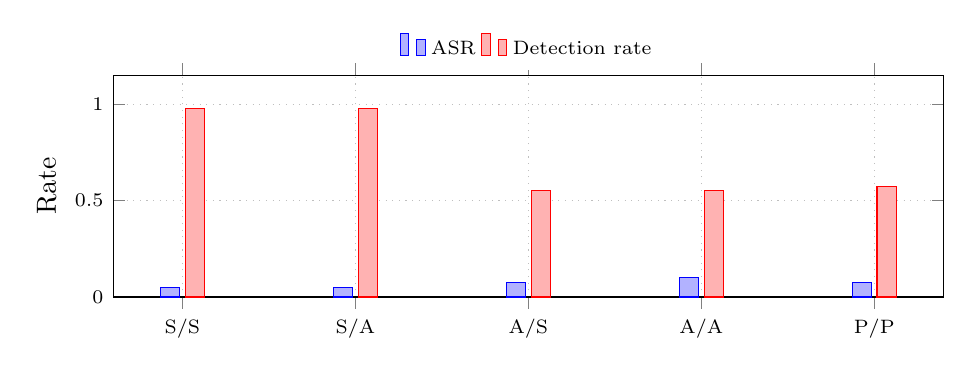
\begin{tikzpicture}
\begin{axis}[
  ybar,
  bar width=7pt,
  width=\columnwidth,
  height=4.4cm,
  ylabel={Rate},
  ymin=0, ymax=1.15,
  symbolic x coords={S/S, S/A, A/S, A/A, P/P},
  xtick=data,
  xticklabel style={font=\scriptsize},
  legend style={font=\scriptsize, at={(0.5,1.02)}, anchor=south, legend columns=2, draw=none},
  yticklabel style={font=\scriptsize},
  grid=major,
  major grid style={dotted,gray!50},
]
\addplot coordinates {(S/S,0.050) (S/A,0.050) (A/S,0.075) (A/A,0.100) (P/P,0.075)};
\addplot coordinates {(S/S,0.975) (S/A,0.975) (A/S,0.550) (A/A,0.550) (P/P,0.575)};
\legend{ASR, Detection rate}
\end{axis}
\end{tikzpicture}
\caption{Ladder outcomes. S\,=\,static, A\,=\,episodic adaptive,
P\,=\,persistent. Adaptive attackers cut detection from $0.975$ to
$0.55$.}
\label{fig:ladder}
\end{figure}


\subsection{Co-Evolution and Stability (RQ3, RQ5, H2)}
CEP is lowest for static/static ($0.36$)---residual variation comes
from environment stochasticity, not from policy updates---and highest
for adaptive/adaptive ($0.50$). Persistent/persistent is classified by
the analysis engine as an \emph{arms race}: late-episode signature
change ($0.52$) exceeds early-episode change ($0.43$), so strategies
do not settle (Fig.~\ref{fig:arms}).

On the persistent run, ASR falls from $0.10$ in the first twenty
episodes to $0.05$ in the last twenty, while mean attacker stealth and
defender vigilance both trend upward. That is the H2 signature:
defenders suppress an initially successful pattern, attackers respond,
neither side freezes. Recovery, when it occurs, is not a return to the
opening strategy; CEP remaining high means the pair is moving through
strategy space.

\begin{figure}[!t]
\centering
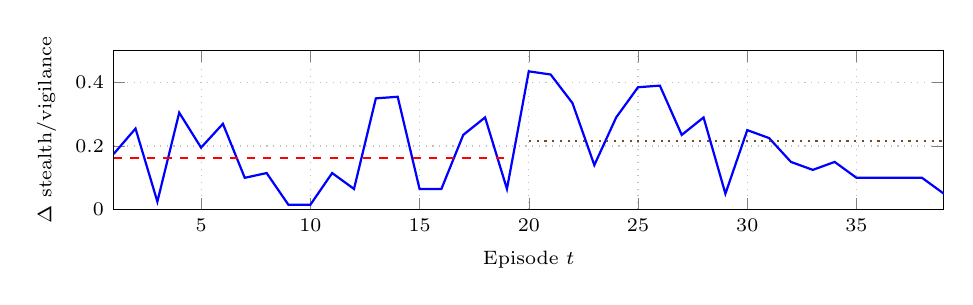
\begin{tikzpicture}
\begin{axis}[
  width=\columnwidth,
  height=3.6cm,
  xlabel={Episode $t$},
  ylabel={$\Delta$ stealth/vigilance},
  xmin=1, xmax=39,
  ymin=0, ymax=0.50,
  xticklabel style={font=\scriptsize},
  yticklabel style={font=\scriptsize},
  label style={font=\scriptsize},
  grid=major,
  major grid style={dotted,gray!50},
]
\addplot+[thick, mark=none] coordinates {(1,0.1750) (2,0.2550) (3,0.0250) (4,0.3050) (5,0.1950) (6,0.2700) (7,0.1000) (8,0.1150) (9,0.0150) (10,0.0150) (11,0.1150) (12,0.0650) (13,0.3500) (14,0.3550) (15,0.0650) (16,0.0650) (17,0.2350) (18,0.2900) (19,0.0650) (20,0.4350) (21,0.4250) (22,0.3350) (23,0.1400) (24,0.2900) (25,0.3850) (26,0.3900) (27,0.2350) (28,0.2900) (29,0.0500) (30,0.2500) (31,0.2250) (32,0.1500) (33,0.1250) (34,0.1500) (35,0.1000) (36,0.1000) (37,0.1000) (38,0.1000) (39,0.0500)};
\addplot+[thick, dashed, mark=none] coordinates {(1,0.1618) (19,0.1618)};
\addplot+[thick, dotted, mark=none] coordinates {(20,0.2162) (39,0.2162)};
\end{axis}
\end{tikzpicture}
\caption{Per-episode parameter change on a representative P/P run (seed~100). Parameter dynamics class: \emph{non convergent}. Distribution over all 54 ladder runs in Table~\ref{tab:dynamics}.}
\label{fig:arms}
\end{figure}


\subsection{Emergence (RQ2, H5)}
Encoded behaviours for the ladder were reconnaissance, privilege
escalation and resource targeting (attacker), plus adaptive monitoring
and dynamic isolation (defender). Post-hoc tagging against the taxonomy
of Section~\ref{sec:problem} found additional behaviours that were
\emph{not} encoded: delayed attack and strategic patience ($240$
occurrences each on the persistent run), strategic resource allocation
($24$), deception and decoy deployment ($7$ each). Delayed attack is
exactly the stealth-pacing wait; it is a strategy discovered from the
detection physics, not an instruction in the objective
(``exfiltrate while minimising detection'' does not mention waiting).
Under the definition of Section~\ref{sec:problem} these are candidate
emergent behaviours. We do not claim they are intelligent; we claim
they were not programmed as scripts and yet arose consistently.

\subsection{What the Ladder Does Not Yet Show}
Communication was disabled, so coalition rate is zero by construction
(H3, H6). ESR is undefined without a paired isolation run on a
population that can talk. LLM capability (H7) is reserved for B3--B5
once the Ollama endpoint is attached. These are not missing controls on
the present claim; they are the next cells of Table~\ref{tab:matrix}.
The claim this section is entitled to is narrower and, we think,
stronger: \emph{the co-evolutionary phenomenon exists already at
one-versus-one, before any society of agents is introduced.}
